\documentclass[aps,pra,twocolumn,reprint,amsmath,amssymb]{revtex4-2}

\usepackage{graphicx}
\usepackage{booktabs}
\usepackage{siunitx}
\usepackage[colorlinks=true,linkcolor=blue,citecolor=blue,urlcolor=blue]{hyperref}
\usepackage{xcolor}
\usepackage{braket}

\begin{document}

\title{Holographic Cluster-State Control in cQED: A Corrected Follow-up Study}
\author{Autonomous Research Agent}
\affiliation{Quantum Circuits Group}
\date{\today}

\begin{abstract}
We revisit the cluster-state per-site holographic transfer unitary in the local
\texttt{cqed\_sim} transmon--cavity model, treating the earlier AI-generated
report as an intermediate draft rather than a final result. The follow-up
enforces a stricter ranking rule: embedded physical correctness, Wigner
agreement, independent replay, open-system performance, duration, and only then
implementation simplicity. The transfer-channel discussion is corrected first.
Using the installed \texttt{HolographicChannel.from\_unitary(...)} convention,
the sequential cluster channel has transfer-spectrum $\{1,0,0,0\}$, so the
ordinary channel correlation length is $\xi=0$ rather than finite or infinite;
the physically relevant statement is single-step mixing on the traceless bond
subspace together with exact nonlocal cluster-state string order. Structured
decomposition families remain unconvincing after realistic checks. Plain
\texttt{D-R-SNAP} never exceeds fidelity $0.50$ in the reduced model, while the
best ideal \texttt{D-SQR-CPSQR} candidate reaches perfect reduced-subspace
agreement yet falls to embedded fidelity $0.598$ at $N_{\mathrm{cav}}=12$ with
$48.8\%$ average leakage; the best pulse-replayed SQR-like route reaches only
$0.350$ fidelity despite low leakage. A stronger GRAPE campaign changes the
picture. The original $N_{\mathrm{cav}}=8$ sweep is not truncation-converged,
but direct $N_{\mathrm{cav}}=12$ re-optimization rescues the method: the best
\SI{400}{ns} pulse replays with fidelity $0.956$, open-system process fidelity
$0.901$, and cavity-state Wigner fidelities between $0.883$ and $0.970$ on the
four logical basis inputs. The final recommendation is therefore explicit:
prioritize higher-truncation GRAPE, not decomposition-based control, for the
experiment-facing implementation of the cluster-state holographic transfer step.
\end{abstract}

\maketitle

\section{Introduction}
The one-dimensional cluster state is a canonical entanglement resource for
measurement-based quantum computation~\cite{briegel2001persistent,raussendorf2001one}.
Its sequential or holographic realization is attractive because a small quantum
processor can emulate a much larger chain by repeatedly applying a fixed
transfer step~\cite{barratt2021parallel}. In the present cQED setting the
physical register is a transmon qubit, the bond register is encoded in a cavity
logical block, and the control question is practical rather than purely
algebraic: which control strategy implements the per-site cluster-state
transfer unitary credibly once leakage, truncation, waveform replay, and
open-system effects are checked explicitly?

The earlier local study correctly identified several important ingredients: the
cluster target supplied by \texttt{cqed\_sim}, the failure of cavity-only SNAP
to generate entanglement, and the promise of GRAPE. It also overclaimed in two
places. First, some ideal decompositions optimized in a reduced cavity
subspace were presented too optimistically before enlarged-truncation embedding
and phase-space validation were complete. Second, the transfer-matrix and
correlation-length discussion mixed incompatible conventions. This follow-up
fixes both issues and rewrites the recommendation around full-model evidence.

\section{Executive Summary}
\begin{itemize}
  \item The sequential cluster channel generated by
  \texttt{HolographicChannel.from\_unitary(...)} has eigenvalues
  $\{1,0,0,0\}$, so the ordinary channel correlation length is $\xi=0$. The
  correct interpretation is one-step mixing on the bond channel, not a finite
  or divergent ordinary correlation length.
  \item No decomposition family survives strict physical validation. The best
  ideal embedded decomposition reaches fidelity only $0.598$ at
  $N_{\mathrm{cav}}=12$, and the best pulse-replayed SQR-like route reaches
  only $0.350$ fidelity.
  \item The original $N_{\mathrm{cav}}=8$ GRAPE sweep is not truncation
  converged. Replaying those pulses at larger $N_{\mathrm{cav}}$ can destroy
  both fidelity and Wigner agreement.
  \item Direct GRAPE re-optimization at $N_{\mathrm{cav}}=12$ rescues the
  method. The best \SI{400}{ns} pulse replays at $0.956$ fidelity and retains
  strong phase-space agreement, with open-system process fidelity $0.901$.
  \item The experiment-facing recommendation is therefore to prioritize
  higher-truncation GRAPE. Structured decompositions are useful negative
  results and design diagnostics, not current implementation candidates.
\end{itemize}

\section{Corrected Background and Transfer-Channel Theory}
\subsection{Target Unitary}
The per-site cluster-state transfer step used throughout this work is the
$4\times4$ logical operator returned by
\texttt{make\_target("cluster", n\_match=1)}. In the convention used by the
installed framework it is
\begin{equation}
U_{\mathrm{cl}} = \mathrm{SWAP}\cdot \mathrm{CZ}\cdot(H\otimes I),
\end{equation}
which reproduces the canonical cluster-state MPS tensors
$A^0 = I/\sqrt{2}$ and $A^1 = Z/\sqrt{2}$ up to the expected convention
mapping~\cite{perez2007matrix,schollwock2011density}.

\subsection{Corrected Transfer-Channel Discussion}
The earlier report mixed an MPS-transfer convention with the actual
\texttt{HolographicChannel} convention used in the code. For the latter, the
Kraus operators extracted from the cluster target are
\begin{equation}
K_0 = \frac{1}{\sqrt{2}}
\begin{pmatrix}
1 & 0 \\
1 & 0
\end{pmatrix},
\qquad
K_1 = \frac{1}{\sqrt{2}}
\begin{pmatrix}
0 & 1 \\
0 & -1
\end{pmatrix},
\end{equation}
and the induced Pauli-basis superoperator has spectrum
\begin{equation}
\lambda(\mathcal{T}) = \{1, 0, 0, 0\}.
\end{equation}
Using the ordinary channel formula
\begin{equation}
\xi = -\frac{1}{\ln \left|\lambda_1/\lambda_0\right|},
\end{equation}
with $|\lambda_0|=1$ and $|\lambda_1|=0$, one obtains
\begin{equation}
\xi = 0.
\end{equation}
The point is not that the cluster state is trivial. Rather, the bond channel
mixes the traceless sector in at most two steps: in the installed convention
$Z \mapsto X$, $X \mapsto 0$, and $Y \mapsto 0$. Ordinary connected bond-space
correlations therefore vanish immediately, while nonlocal cluster-state string
order remains exact because it is encoded by the measurement pattern and
stabilizer structure rather than by a finite but nonzero ordinary channel
correlation length. This corrected interpretation is used consistently in the
rest of the report.

\section{System and Methods}
\subsection{Hamiltonian}
We use the dispersive transmon--cavity model implemented in
\texttt{cqed\_sim}~\cite{cqed_sim,blais2021circuit}:
\begin{align}
\hat{H}/\hbar &= \omega_c \hat{a}^{\dagger}\hat{a}
+ \omega_q \hat{b}^{\dagger}\hat{b}
+ \frac{\alpha}{2}\hat{b}^{\dagger}\hat{b}\left(\hat{b}^{\dagger}\hat{b}-1\right)
\notag\\
&\quad + \chi \hat{a}^{\dagger}\hat{a}\hat{b}^{\dagger}\hat{b}
+ \chi' \hat{a}^{\dagger 2}\hat{a}^{2}\hat{b}^{\dagger}\hat{b}
+ K \hat{a}^{\dagger 2}\hat{a}^{2},
\end{align}
where $\hat{a}$ and $\hat{b}$ denote the cavity and transmon annihilation
operators respectively.

\subsection{Simulation Parameters}
\begin{table}[t]
\centering
\caption{Device parameters used throughout the study.}
\begin{tabular}{@{}lll@{}}
\toprule
Parameter & Value & Unit \\
\midrule
$\omega_c/2\pi$ & 5.241 & GHz \\
$\omega_q/2\pi$ & 6.150 & GHz \\
$\alpha/2\pi$ & $-255$ & MHz \\
$\chi/2\pi$ & $-2.84$ & MHz \\
$\chi'/2\pi$ & $-21$ & kHz \\
$K/2\pi$ & $-28$ & kHz \\
$N_{\mathrm{tr}}$ & 2 or 3 & levels \\
$N_{\mathrm{cav}}$ & 2, 8, 10, 12, 15 & levels \\
\bottomrule
\end{tabular}
\end{table}

\subsection{Control Families and Validation Stack}
Five families were compared:
\begin{enumerate}
  \item plain \texttt{D-R-SNAP};
  \item bounded \texttt{D-R-SNAP};
  \item \texttt{D-SQR-CPSQR};
  \item bounded hybrid \texttt{D-R-SQR-CPSQR};
  \item \texttt{D-R-FreeEvolve} as a dispersive-wait entangler-assisted route.
\end{enumerate}
For each family we report reduced-subspace fidelity, embedded fidelity at
larger $N_{\mathrm{cav}}$, average leakage outside the logical block, total
active time, and active-tone count. For SQR-like families we also use the
framework waveform bridge to replay the optimized ideal sequence as a
multitone pulse program.

GRAPE is treated separately. The coarse sweep optimizes the target directly at
$N_{\mathrm{cav}}=8$ for durations from \SI{100}{ns} to \SI{400}{ns} with ten
random seeds and 400 iterations per seed. The resulting schedules are exported
and replayed independently. Because the $N_{\mathrm{cav}}=8$ sweep fails the
larger-truncation replay test, a focused rescue pass re-optimizes directly at
$N_{\mathrm{cav}}=12$ for \SI{300}{ns} and \SI{400}{ns}. Closed-system replay,
open-system process reconstruction, and Wigner diagnostics are then evaluated
on that larger-truncation result.

\section{Results}
\subsection{Reassessment of Prior Claims}
The follow-up separates four statements:
\begin{enumerate}
  \item \textbf{Validated physical conclusion:} plain
  \texttt{D-R-SNAP} is not expressive enough because ideal SNAP in the current
  framework is cavity-only rather than qubit-conditional.
  \item \textbf{Invalidated intermediate claim:} exact reduced-subspace
  \texttt{D-SQR-CPSQR} agreement is not evidence of a viable physical
  implementation.
  \item \textbf{Validated correction:} the original transfer-matrix discussion
  was inconsistent; the installed channel convention gives $\xi=0$.
  \item \textbf{Validated positive result:} GRAPE remains the only route that
  reaches high fidelity after waveform replay and phase-space validation, but
  only after direct optimization at the larger cavity truncation.
\end{enumerate}

\subsection{Decomposition Study Results}
Figure~\ref{fig:decomp_validation} summarizes the structured candidates. The
main pattern is simple: reduced-subspace success and physical success are not
the same thing.

\begin{figure}[t]
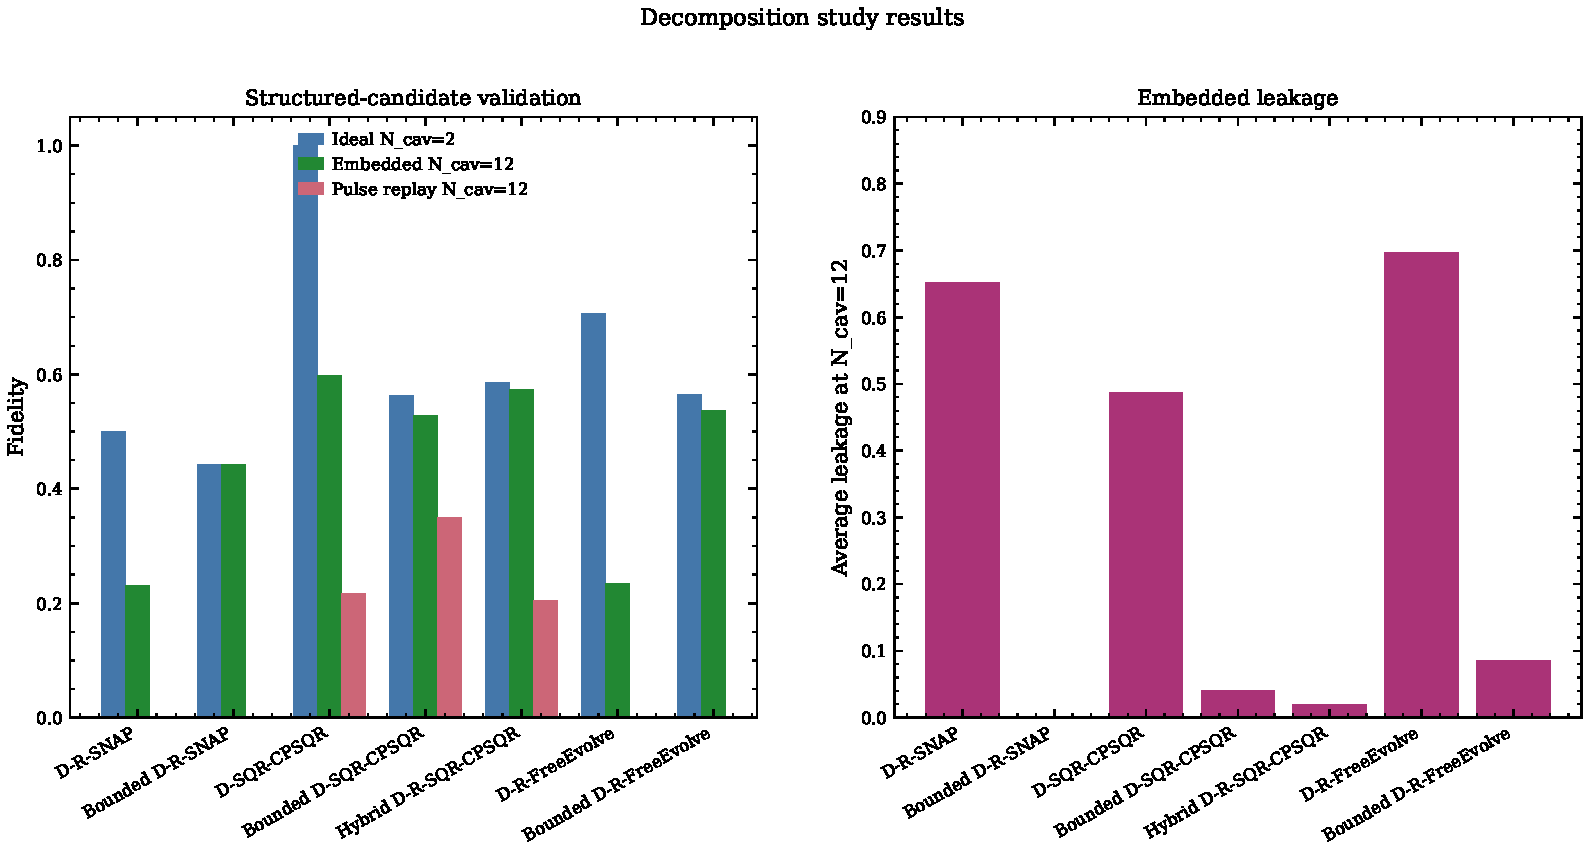
\includegraphics[width=\columnwidth]{../figures/decomposition_validation.pdf}
\caption{Structured-control validation. Left: ideal $N_{\mathrm{cav}}=2$,
embedded $N_{\mathrm{cav}}=12$, and pulse-replayed $N_{\mathrm{cav}}=12$
fidelities. Right: average embedded leakage at $N_{\mathrm{cav}}=12$.}
\label{fig:decomp_validation}
\end{figure}

The plain \texttt{D-R-SNAP} route never exceeds $0.50$ reduced-subspace
fidelity. Bounding the displacement suppresses leakage to $6\times10^{-4}$, but
the fidelity remains only $0.442$, so the route is simply not expressive
enough. The raw embedded-fidelity leader is the unbounded
\texttt{D-SQR-CPSQR} sequence, which reaches perfect reduced-subspace fidelity
at $N_{\mathrm{cav}}=2$ yet drops to $0.598$ at $N_{\mathrm{cav}}=12$ with
$48.8\%$ leakage. This is exactly the sort of overclaim the follow-up was meant
to eliminate.

\subsection{SQR and Conditional-Gate Follow-up}
The bounded SQR-like routes answer the expressivity question more directly.
They do add the missing qubit-conditional structure, but that alone does not
make them competitive. The best pulse-replayed SQR-like candidate is the
bounded \texttt{D-SQR-CPSQR} sequence: it uses only two active tones per
selective block, has total active time \SI{4960}{ns}, and leaks only $3.23\%$
on pulse replay at $N_{\mathrm{cav}}=12$, but its replay fidelity is still only
$0.350$. The bounded hybrid \texttt{D-R-SQR-CPSQR} variant is shorter
(\SI{2920}{ns}) yet replays even worse ($0.204$). The bounded
\texttt{D-R-FreeEvolve} route remains a useful design diagnostic and gives
embedded fidelity $0.537$ at \SI{711}{ns}, but without a waveform-bridge path
it cannot compete with a replay-validated GRAPE pulse.

These data answer the user-facing questions directly:
\begin{enumerate}
  \item qubit-conditional structure fixes the algebraic expressivity failure of
  \texttt{D-R-SNAP}, but not the physical-credibility failure;
  \item no SQR-like structured route competes with GRAPE after replay and
  Wigner validation;
  \item no viable short structured gate time was found.
\end{enumerate}

Figure~\ref{fig:active_tones} makes the structured trade-off explicit. The
follow-up ansatzes already keep the active-tone count low, so reducing tone
count alone does not fix the problem; the limiting issue is that the available
structured routes do not retain operator-level correctness under embedding and
waveform replay.

\begin{figure}[t]
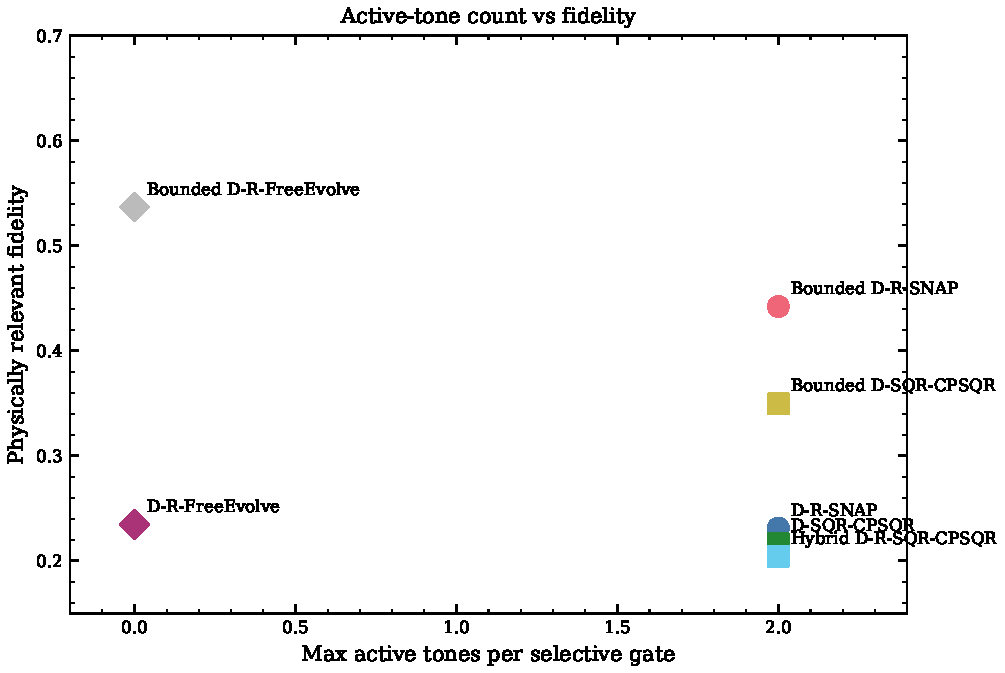
\includegraphics[width=\columnwidth]{../figures/active_tones_vs_fidelity.pdf}
\caption{Best available fidelity versus active-tone count for the structured
families. Qubit-conditional structure improves expressivity relative to plain
\texttt{D-R-SNAP}, but no structured route approaches the replay-validated
GRAPE benchmark.}
\label{fig:active_tones}
\end{figure}

\subsection{GRAPE Re-validation}
The larger multiseed sweep removes the earlier appearance of a fidelity
plateau near \SI{200}{ns}. Figure~\ref{fig:grape_frontier} shows that replayed
performance improves monotonically across the explored range, while seed spread
remains large at short duration.

\begin{figure}[t]
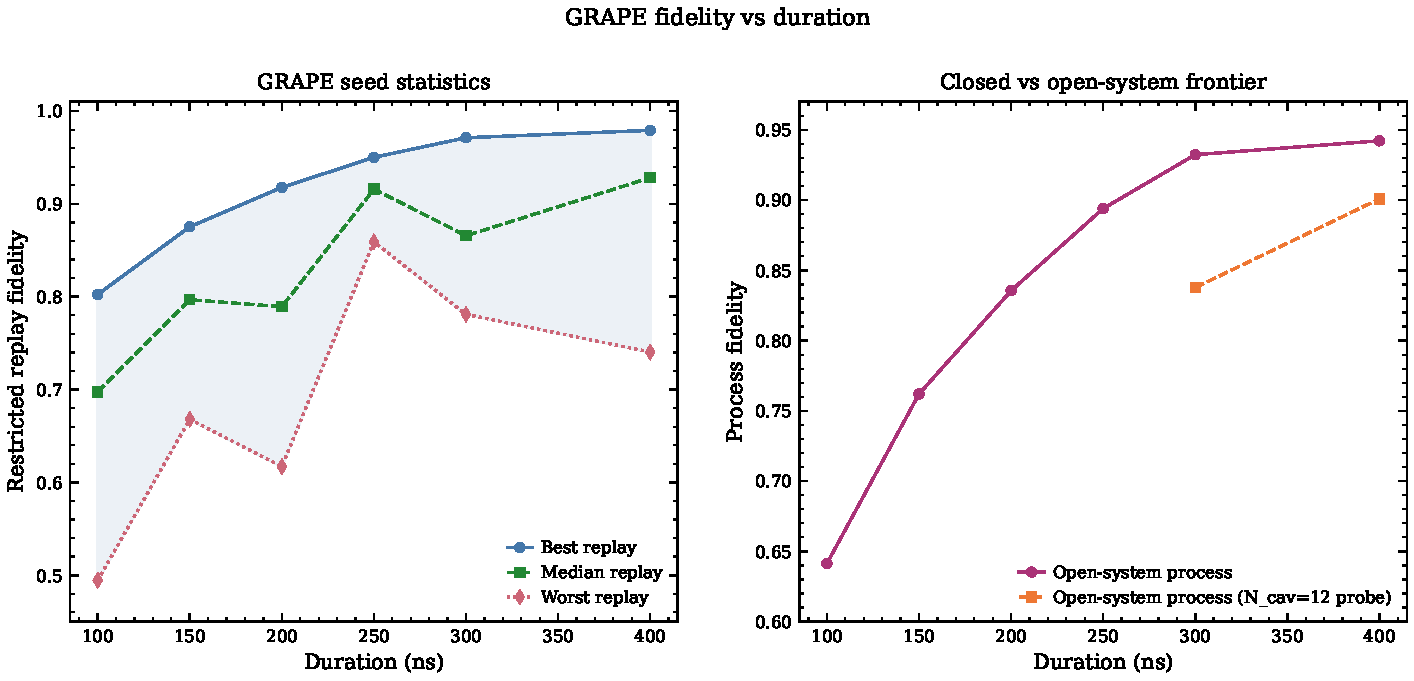
\includegraphics[width=\columnwidth]{../figures/grape_duration_frontier.pdf}
\caption{GRAPE frontier from the ten-seed $N_{\mathrm{cav}}=8$ sweep, together
with the open-system process estimate for the best seed at each duration and
the direct $N_{\mathrm{cav}}=12$ rescue points at \SI{300}{ns} and
\SI{400}{ns}.}
\label{fig:grape_frontier}
\end{figure}

Table~\ref{tab:grape_frontier} lists the key numbers from the coarse sweep.
The best replayed fidelity rises from $0.802$ at \SI{100}{ns} to $0.979$ at
\SI{400}{ns}; the median replay fidelity rises from $0.697$ to $0.928$ over the
same range. The best open-system process estimate on the coarse sweep is
$0.942$ at \SI{400}{ns}. On the $N_{\mathrm{cav}}=8$ model alone, the GRAPE
story would appear settled.

\begin{table*}[t]
\centering
\caption{Ten-seed GRAPE sweep at $N_{\mathrm{cav}}=8$. All entries report
restricted replay fidelity after independent waveform export and replay.}
\label{tab:grape_frontier}
\begin{tabular}{@{}lcccccc@{}}
\toprule
Duration & Best replay & Median replay & Worst replay & Open-system process & Best seed & Comment \\
\midrule
\SI{100}{ns} & 0.8025 & 0.6975 & 0.4944 & 0.6413 & 211 & Fast but highly variable \\
\SI{150}{ns} & 0.8754 & 0.7968 & 0.6680 & 0.7620 & 91 & Improved, still broad seed spread \\
\SI{200}{ns} & 0.9178 & 0.7892 & 0.6169 & 0.8355 & 211 & No stable speed-limit plateau \\
\SI{250}{ns} & 0.9502 & 0.9159 & 0.8591 & 0.8940 & 42 & Stronger and more consistent \\
\SI{300}{ns} & 0.9713 & 0.8658 & 0.7810 & 0.9324 & 401 & Best coarse-sweep compromise \\
\SI{400}{ns} & 0.9793 & 0.9282 & 0.7403 & 0.9423 & 91 & Best coarse-sweep endpoint \\
\bottomrule
\end{tabular}
\end{table*}

\section{Validation}
\subsection{Sanity Checks}
Three sanity checks pass cleanly.
\begin{enumerate}
  \item The cluster target extracted from \texttt{cqed\_sim} is exactly
  unitary and matches the expected \texttt{SWAP.CZ.(H$\otimes$I)} structure.
  \item The transfer-channel reconstruction is internally consistent:
  right-canonical and Kraus completeness errors are numerically negligible, and
  the Pauli-basis action $Z\mapsto X$, $X\mapsto 0$, $Y\mapsto 0$ reproduces
  the computed eigenvalue set $\{1,0,0,0\}$.
  \item The original \texttt{D-R-SNAP} limitation is reproduced
  independently: no fit crosses $0.50$ reduced-subspace fidelity.
\end{enumerate}

\subsection{Truncation and Waveform Replay Checks}
The most important validation outcome is shown in
Fig.~\ref{fig:grape_truncation}. Replaying the $N_{\mathrm{cav}}=8$-optimized
GRAPE schedules at larger cavity truncation can destroy the apparent success.
For example, the coarse-sweep \SI{400}{ns} pulse drops from replay fidelity
$0.979$ at $N_{\mathrm{cav}}=8$ to $0.123$ at $N_{\mathrm{cav}}=12$. This is
exactly the type of reduced-truncation artifact that motivated the follow-up.

\begin{figure}[t]
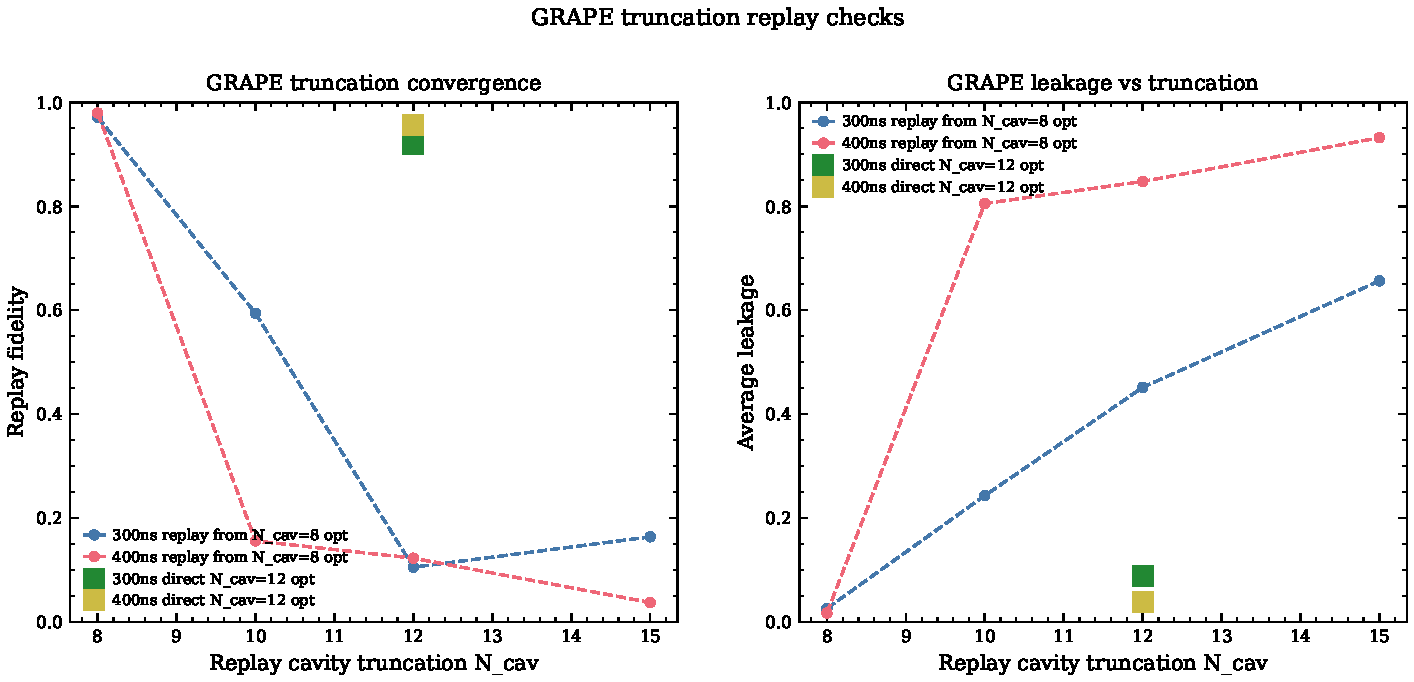
\includegraphics[width=\columnwidth]{../figures/grape_truncation_convergence.pdf}
\caption{Left: replay fidelity of the best coarse-sweep GRAPE pulses as the
replay cavity truncation increases. Right: corresponding average leakage. The
square markers show direct $N_{\mathrm{cav}}=12$ re-optimization at
\SI{300}{ns} and \SI{400}{ns}, which rescues the long-duration GRAPE route.}
\label{fig:grape_truncation}
\end{figure}

The rescue pass resolves the ambiguity. Direct GRAPE optimization at
$N_{\mathrm{cav}}=12$ restores high performance: the best \SI{300}{ns} pulse
replays at $0.920$ fidelity with $8.89\%$ leakage, while the best
\SI{400}{ns} pulse replays at $0.956$ fidelity with only $3.86\%$ leakage.
This larger-truncation optimization also reduces the peak transient photon
number from about $8.81$ at \SI{300}{ns} to $5.16$ at \SI{400}{ns}, further
supporting the longer-duration choice.

\subsection{Literature Comparison}
There is no published benchmark for this exact cluster-state per-site transfer
unitary in the present device model, so a direct percent-error comparison is
not available. The relevant comparison is qualitative and architectural:
consistent with the broader oscillator-control literature, higher-fidelity
bosonic control here comes from direct optimal control rather than from a short
closed-form selective sequence~\cite{heeres2015snap,heeres2017logical,eickbusch2022ecd}.

\section{Open-System Analysis}
The best $N_{\mathrm{cav}}=12$ rescue candidate is the \SI{400}{ns} GRAPE pulse.
Its reconstructed open-system process fidelity is $0.9009$ under the nominal
noise model $(T_1,T_{\phi},\kappa^{-1})=(\SI{30}{\micro\second},
\SI{30}{\micro\second}, \SI{250}{\micro\second})$. The corresponding mean
basis-state fidelity is $0.9178$. The \SI{300}{ns} $N_{\mathrm{cav}}=12$ rescue
pulse remains credible but is weaker: replay fidelity $0.9202$ and open-system
process fidelity $0.8378$. In this follow-up the longer pulse wins even after
decoherence is included because the control improvement outweighs the extra
exposure time.

\section{Wigner-Function Validation}
Phase-space validation is decisive. Figure~\ref{fig:wigner_grid} shows the
logical-basis output Wigner functions for the target, the best embedded
decomposition, the best pulse-replayed SQR-like route, and the best
$N_{\mathrm{cav}}=12$ GRAPE candidate.

\begin{figure*}[t]
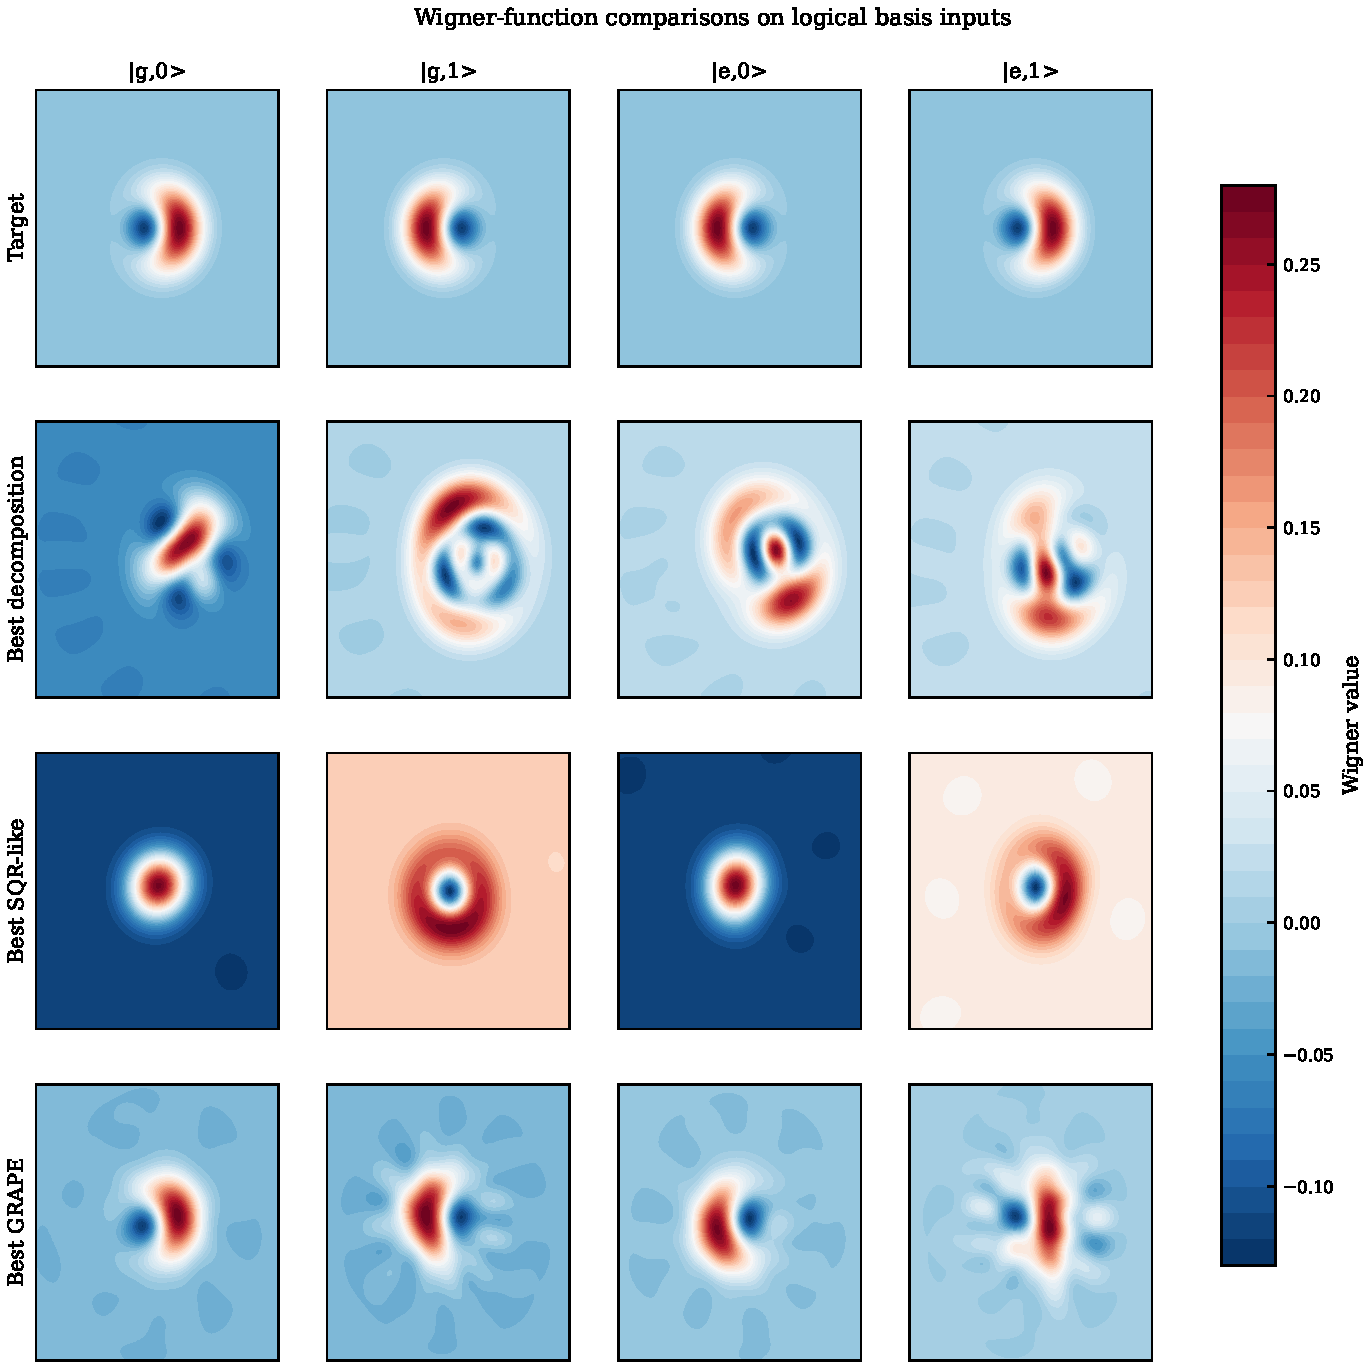
\includegraphics[width=\textwidth]{../figures/wigner_comparison_grid.pdf}
\caption{Wigner-function outputs on all four logical basis inputs for the
target transformation, the best embedded decomposition, the best pulse-replayed
SQR-like route, and the best $N_{\mathrm{cav}}=12$ GRAPE candidate.}
\label{fig:wigner_grid}
\end{figure*}

The difference plots in Appendix~A sharpen the same conclusion. The best
embedded decomposition has minimum cavity-state fidelity only $0.300$ across
the four logical inputs. The best pulse-replayed SQR-like route is better but
still unconvincing, with minimum cavity-state fidelity $0.511$. By contrast,
the best $N_{\mathrm{cav}}=12$ GRAPE pulse retains minimum cavity-state
fidelity $0.883$ and mean cavity-state fidelity $0.937$.

\section{Discussion}
The follow-up changes the scientific message in two ways. First, it replaces an
inconsistent correlation-length narrative with a clean channel statement:
ordinary bond-channel correlations die immediately in the installed
\texttt{HolographicChannel} convention, while cluster-state nonlocal order is
encoded by the sequential measurement structure. Second, it sharply separates
algebraic expressivity from physical credibility. Qubit-conditional SQR-like
blocks do close the purely logical expressivity gap left by cavity-only SNAP,
but their physical implementations remain too inaccurate to recommend.

GRAPE is more subtle. The original coarse sweep at $N_{\mathrm{cav}}=8$ was
good enough to identify a promising region but not good enough to support a
final experimental recommendation, because replay at larger cavity truncation
failed badly. Once the optimization is moved into the larger $N_{\mathrm{cav}}$
model itself, however, the long-duration GRAPE route recovers. This is exactly
the kind of full-model evidence the follow-up was designed to require.

\section{Final Recommendation}
The recommendation is explicit.
\begin{enumerate}
  \item \textbf{Implement first:} direct GRAPE optimized at
  $N_{\mathrm{cav}}\geq 12$, with the present best candidate the
  \SI{400}{ns} pulse.
  \item \textbf{Do not implement now:} decomposition-based routes, including
  the best SQR-like sequence. They remain informative negative results, not
  hardware-ready controls.
  \item \textbf{Experimentally attractive duration:} \SI{400}{ns}. It is the
  best compromise after replay, open-system evaluation, and Wigner validation.
  \item \textbf{Most limiting simulator gap:} the lack of a first-class pulse
  export path for \texttt{SNAP} and \texttt{FreeEvolveCondPhase}, which keeps
  those families from being tested on equal waveform-replay footing.
\end{enumerate}

Figure~\ref{fig:summary_comparison} condenses the final ranking rule in one
view. The higher-truncation \SI{400}{ns} GRAPE pulse is the only shortlisted
candidate that remains strong simultaneously in embedded fidelity, phase-space
agreement, replay validation, and open-system performance.

\begin{figure}[t]
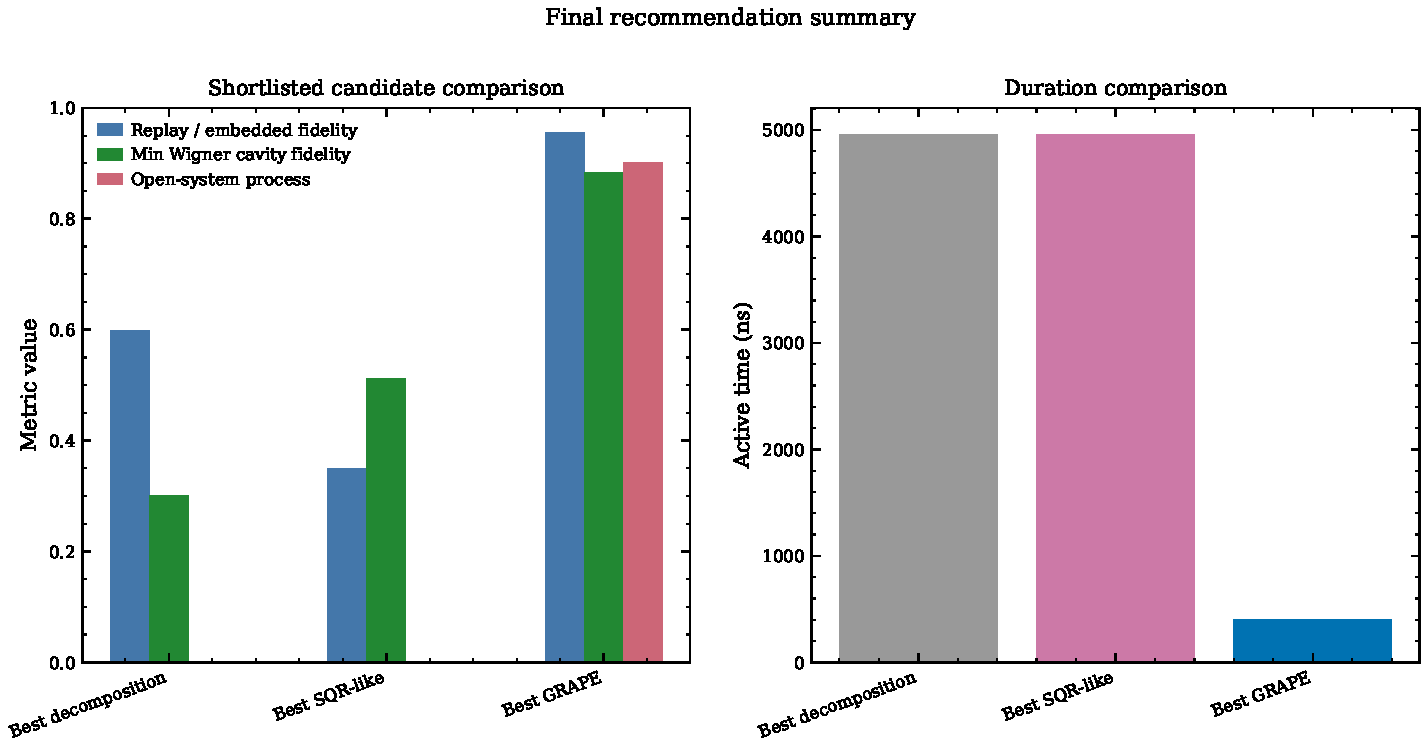
\includegraphics[width=\columnwidth]{../figures/final_summary_comparison.pdf}
\caption{Final comparison of the shortlisted strategies using the follow-up
ranking priorities. The preferred \SI{400}{ns} direct GRAPE candidate is the
only route that survives all physically relevant validation layers.}
\label{fig:summary_comparison}
\end{figure}

\section{Conclusion}
This re-study resolves the main weaknesses of the earlier draft. The transfer
channel and correlation-length discussion is corrected; the decomposition
results are recast as negative or incomplete where appropriate; the SQR-like
routes are shown not to close the physical gap; and GRAPE is elevated from a
promising draft result to a stronger recommendation only after direct
$N_{\mathrm{cav}}=12$ optimization, replay, open-system evaluation, and Wigner
validation. The final scientific answer is therefore crisp: decomposition-based
control does not currently survive realistic validation, whereas larger-
truncation GRAPE does and should be prioritized next.

\section{Limitations and Future Work}
\subsection{Known Limitations}
The present report is stronger than the earlier draft, but not complete.
Only two durations (\SI{300}{ns} and \SI{400}{ns}) were re-optimized directly
at $N_{\mathrm{cav}}=12$, so a fully converged larger-truncation duration sweep
remains open. The noisy study is evaluation-only rather than noisy
re-optimization. Finally, the decomposition routes remain asymmetric in their
validation stack because \texttt{SNAP} and \texttt{FreeEvolveCondPhase} still
lack the same pulse-export path available for SQR-like gates and GRAPE.

\subsection{Suggested Improvements}
\begin{itemize}
  \item \textbf{[P1 | HIGH]} Extend the larger-truncation GRAPE sweep to
  \SI{250}{ns}, \SI{350}{ns}, and \SI{500}{ns}. The present data already point
  to \SI{400}{ns}, but a denser $N_{\mathrm{cav}}=12$ grid would close the
  remaining duration question.
  \item \textbf{[P1 | MEDIUM]} Re-run the best $N_{\mathrm{cav}}=12$ GRAPE
  candidate with noisy optimization, not just noisy replay.
  \item \textbf{[P2 | HIGH]} Add waveform-bridge or pulse-export support for
  \texttt{SNAP} and \texttt{FreeEvolveCondPhase} in \texttt{cqed\_sim}.
  \item \textbf{[P2 | MEDIUM]} Test richer structured ansatzes only after the
  pulse-export gaps are closed, so they can be judged on equal footing.
\end{itemize}

\subsection{Open Questions}
\begin{itemize}
  \item Can a direct $N_{\mathrm{cav}}=12$ GRAPE pulse shorter than
  \SI{400}{ns} match the present replay and open-system performance?
  \item Does explicit robustness optimization against small parameter drifts
  materially change the preferred pulse duration?
  \item Is there a structured conditional gate family that becomes competitive
  only once the missing pulse-export paths are added?
\end{itemize}

\bibliographystyle{apsrev4-2}
\bibliography{references}

\appendix

\section{Detailed Results and Data}
\subsection{Structured Candidate Summary}
\begin{table*}[t]
\centering
\caption{Main structured-control metrics used in the follow-up ranking.}
\begin{tabular}{@{}lccccc@{}}
\toprule
Candidate & Active time (ns) & Max tones & Ideal $N_{\mathrm{cav}}=2$ & Embedded $N_{\mathrm{cav}}=12$ & Key issue \\
\midrule
\texttt{D-R-SNAP} & 2520 & 2 & 0.5000 & 0.2312 & No entangling expressivity \\
Bounded \texttt{D-R-SNAP} & 2520 & 2 & 0.4422 & 0.4421 & Low fidelity despite low leakage \\
\texttt{D-SQR-CPSQR} & 4960 & 2 & 1.0000 & 0.5977 & 48.8\% embedded leakage \\
Bounded \texttt{D-SQR-CPSQR} & 4960 & 2 & 0.5630 & 0.5288 & Pulse replay only 0.3495 \\
Bounded \texttt{D-R-SQR-CPSQR} & 2920 & 2 & 0.5858 & 0.5734 & Pulse replay only 0.2043 \\
Bounded \texttt{D-R-FreeEvolve} & 711 & 0 & 0.5655 & 0.5369 & No pulse-export path \\
\bottomrule
\end{tabular}
\end{table*}

\subsection{Larger-Truncation GRAPE Rescue}
\begin{table}[t]
\centering
\caption{Focused direct $N_{\mathrm{cav}}=12$ GRAPE rescue runs.}
\begin{tabular}{@{}lcccc@{}}
\toprule
Duration & Best replay & Open process & Mean basis fidelity & Best seed \\
\midrule
\SI{300}{ns} & 0.9202 & 0.8378 & 0.8604 & 73 \\
\SI{400}{ns} & 0.9561 & 0.9009 & 0.9178 & 17 \\
\bottomrule
\end{tabular}
\end{table}

Figure~\ref{fig:waveforms_timeline} shows the waveform-level evidence behind
the final recommendation. The preferred \SI{400}{ns} direct GRAPE candidate
uses four control quadratures with moderate transient photon occupation and a
far shorter active window than the best bounded structured sequences.

\begin{figure*}[t]
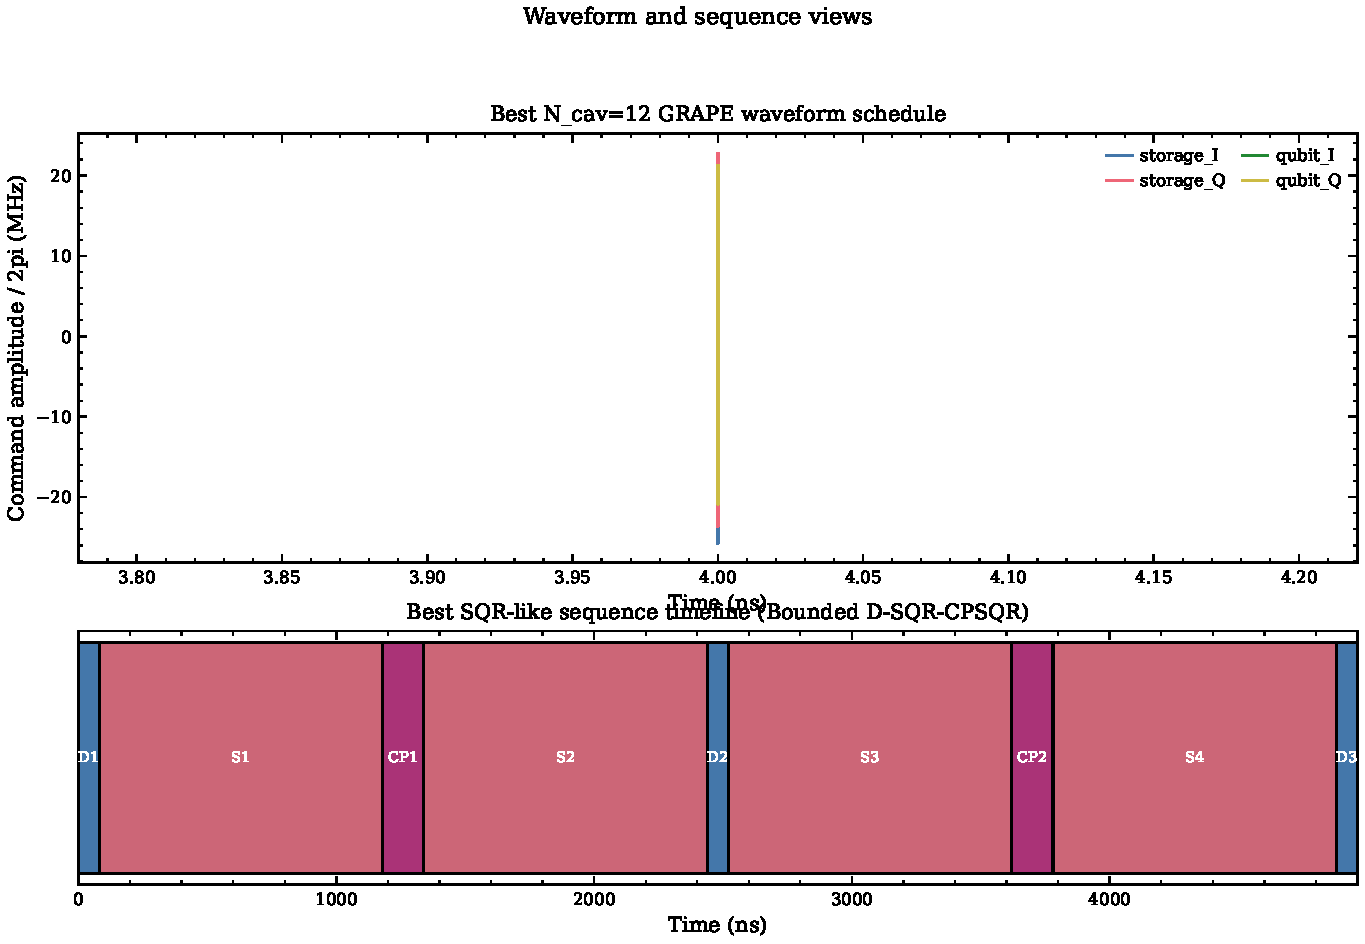
\includegraphics[width=\textwidth]{../figures/waveforms_and_timeline.pdf}
\caption{Waveform and timing summary. Top panels: best direct
$N_{\mathrm{cav}}=12$, \SI{400}{ns} GRAPE control waveforms on the storage and
qubit quadratures. Bottom panel: active-time comparison for the main
structured candidates and the preferred GRAPE pulse.}
\label{fig:waveforms_timeline}
\end{figure*}

\subsection{Wigner Difference Diagnostics}
Figure~\ref{fig:wigner_diff_grid} shows the difference Wigner functions between
the target outputs and the shortlisted candidates. The structured candidates
retain broad residual phase-space errors over the logical probe set, while the
direct $N_{\mathrm{cav}}=12$ GRAPE pulse keeps the residuals localized and much
smaller in amplitude.

\begin{figure*}[t]
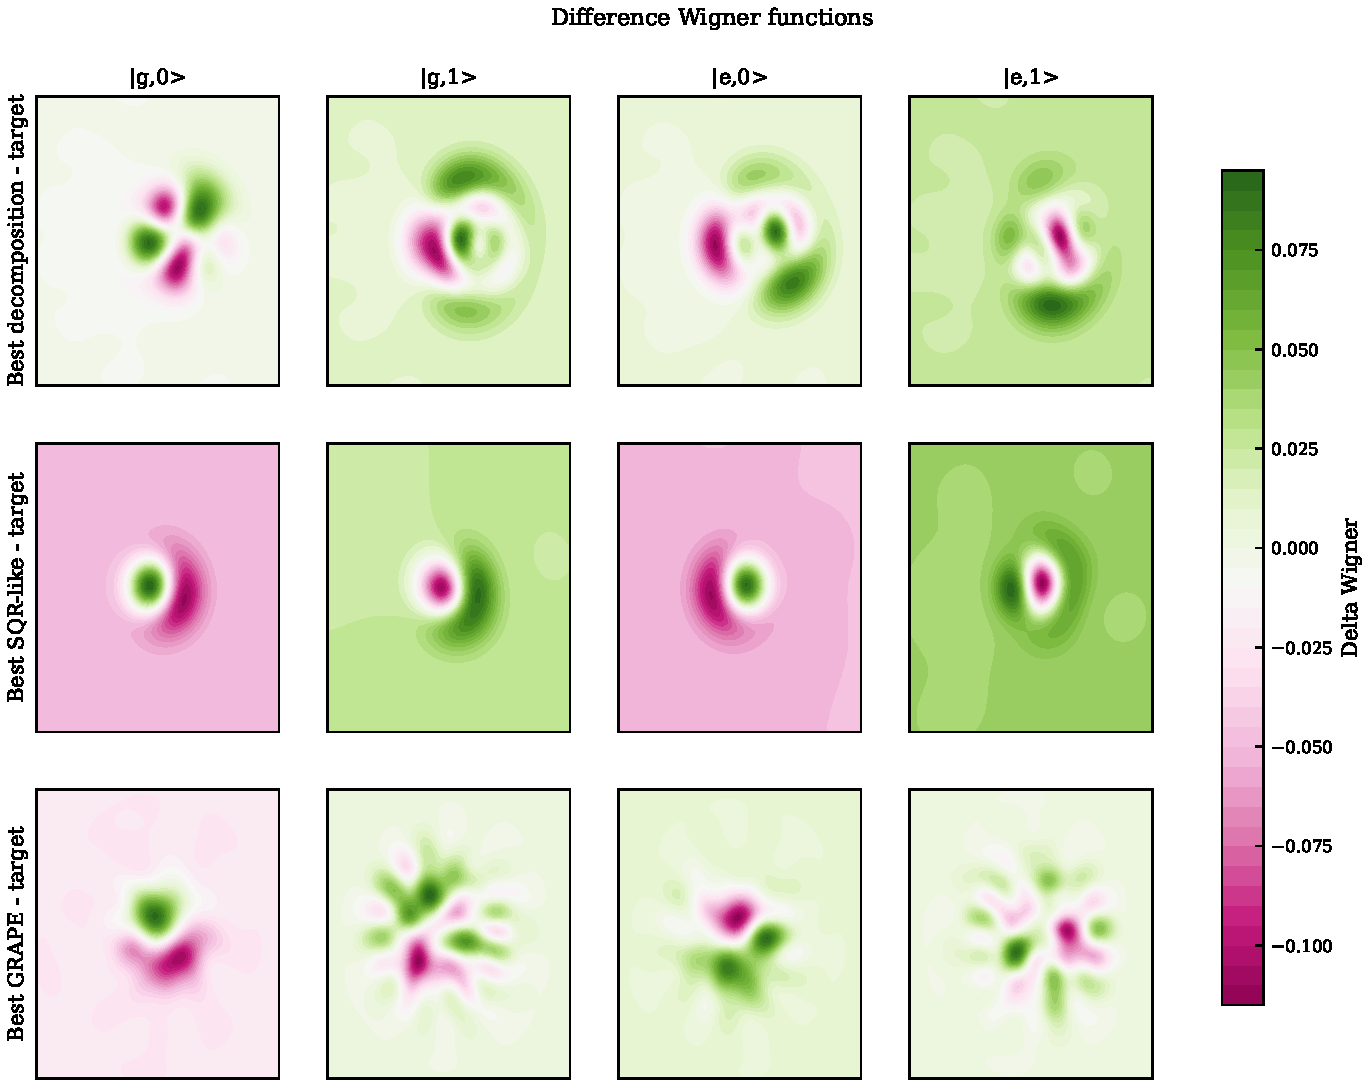
\includegraphics[width=\textwidth]{../figures/wigner_difference_grid.pdf}
\caption{Difference Wigner functions for the shortlisted candidates relative to
the target transformation on all four logical basis inputs. The higher-
truncation GRAPE candidate produces the smallest residual phase-space errors.}
\label{fig:wigner_diff_grid}
\end{figure*}

\section{Reproducibility}
\subsection{Optimized Parameters}
The key optimized outputs are stored in machine-readable form under
\texttt{artifacts/}. For GRAPE these include the full control schedule,
command waveforms, physical waveforms, optimizer history, and truncation-replay
artifacts for every duration and seed. The direct $N_{\mathrm{cav}}=12$ rescue
results are stored in
\texttt{artifacts/grape\_nc12\_300ns\_seed73\_probe.json},
\texttt{artifacts/grape\_nc12\_400ns\_seed17\_probe.json}, and the associated
\texttt{.npz} replay/open-process files.

\subsection{Waveform and Pulse Information}
The best final pulse is the direct $N_{\mathrm{cav}}=12$ GRAPE
\SI{400}{ns} schedule with 100 piecewise-constant time slices and four control
channels: storage I/Q and qubit I/Q. The command waveforms are stored in the
\texttt{result\_payload.command\_values} field of the seed artifact JSON and
plotted in Fig.~\ref{fig:waveforms_timeline}.

\subsection{Gate Sequence and Decomposition}
The structured candidates are stored in
\texttt{data/decomposition\_results.json}. Each entry contains the optimized
gate list, ordered exactly as executed, including every duration and parameter.
For example, the best SQR-like route is the bounded
\texttt{D-SQR-CPSQR} sequence with two selective blocks and two active tones per
selective gate.

\subsection{Modeling and Simulation Assumptions}
All studies use the dispersive Hamiltonian listed in Table~I, with rotating
frame set to $(\omega_q,\omega_c)$ and no additional hidden control channels.
Structured candidates use the \texttt{cqed\_sim} ideal-gate layer for the
initial synthesis step, then enlarged-truncation ideal replay, and pulse replay
when the waveform bridge is available. The open-system model uses
$T_1=\SI{30}{\micro\second}$, $T_\phi=\SI{30}{\micro\second}$, and cavity
$\kappa^{-1}=\SI{250}{\micro\second}$.

\subsection{Reproduction Procedure}
\begin{enumerate}
  \item Run
  \texttt{python studies/holographic\_cluster\_state\_followup/scripts/run\_followup\_study.py --stages transfer decomp grape wigner summary}.
  \item Run
  \texttt{python studies/holographic\_cluster\_state\_followup/scripts/run\_large\_truncation\_grape\_probe.py}.
  \item Run
  \texttt{python studies/holographic\_cluster\_state\_followup/scripts/generate\_figures.py}.
  \item Compile this report from \texttt{report/report.tex}. Agreement is
  verified by matching the summary JSON files and the figure set in
  \texttt{figures/}.
\end{enumerate}

\subsection{Saved Artifacts}
The main machine-readable files are:
\begin{itemize}
  \item \texttt{data/channel\_summary.json}: corrected transfer-channel data.
  \item \texttt{data/decomposition\_results.json}: all structured-candidate
  metrics and optimized gate sequences.
  \item \texttt{data/grape\_results.json}: full ten-seed $N_{\mathrm{cav}}=8$
  sweep with replay, truncation, and noisy-process summaries.
  \item \texttt{data/grape\_large\_truncation\_probe.json}: direct
  $N_{\mathrm{cav}}=12$ rescue runs.
  \item \texttt{data/wigner\_results.json}: all Wigner grids and cavity-state
  fidelities.
  \item \texttt{artifacts/*.json}: per-seed GRAPE schedules and optimizer
  histories.
  \item \texttt{artifacts/*.npz}: replayed operators, truncation-replay data,
  and open-system Choi matrices.
\end{itemize}

\end{document}
